\documentclass{scrreprt}
\usepackage{geometry}
\geometry{a4paper}

\usepackage[english]{babel}
\usepackage[utf8]{inputenc}
\usepackage[parfill]{parskip}
\usepackage{amssymb}
\usepackage{amsmath,mleftright}
\usepackage{euler}
\usepackage{xparse}

\counterwithout{footnote}{chapter}
\usepackage{graphicx}
\graphicspath{ {./images} }

\title{MOBA3 Control System}
\subtitle{System Design Specification and Documentation}
\author{Andreas Wälchli}

\hyphenation{trans-ceiver}
\hyphenation{trans-ceivers}

\newcommand\n{\char`\\n}

\begin{document}
\maketitle

\tableofcontents

\chapter{Introduction}
The \textsc{Moba3} control system is designed as a replacement for previous control systems.
This upgrade is a complete rework and removes all legacy components from previous versions.
Such a step is obviously not taken without careful consideration.

This document outlines the history of the \textsc{Moba} control systems and presents the rationale behind the move to a completely new system.
It also presents the design goals for the new \textsc{Moba3} system.
Finally it serves as a full specification and documentation of both the hardware and software.

The documentation does not provide detailed information about the software implementation.
It only aims to specify the communications interfaces.
Details about software internals and precise decoder operation are deliberately excluded.



\section{Historical Context}
During the construction of the current model railway the decision was made to use traditional analog control for the trains.
Many models were not yet equipped with digital decoders and a retrofit would have been exceedingly expensive.
Since no industry standard digital solution was used for the train control, the decision was made to design and construct a custom digital control solution for all other components of the railway.
This solution would provide push button based control from a schematic control board to control all switches, signals and all lighting.

\subsection{MOBA1}
A first design used custom control and decoder boards based on the PIC16F527 microcontroller.
The entire railway was divided into 5 sectors:

\emph{Shadow station}, \emph{left entry to main station}, \emph{right entry to main station}, \emph{track switches} and \emph{lighting}.

Each sector had a \emph{master} board embedded in the control board that controlled up to 16 push buttons, 16 LEDs on the control board and continuously transmitted a single 8-bit data packet to the decoders in the railway.
This packet did not encode commands but rather a fixed \emph{desired state}.
Each decoder would receive the current state data and check what modifications to its own outputs had to be done to conform to that state.
As a consequence each decoder required bespoke decoding logic.
The data also had to be encoded very efficiently to fit the fixed-length packet.
The sector \emph{right entry to main station} for example controlled 6 switches, 2 entry signals, 4 exit signals and could drive up to 2 independent paths at once.

Each packet contained a single \emph{even parity bit} was packed between start and end marker bits:

\begin{table}[ht!]
\centering
\begin{tabular}{ | c | c | c | c | }
\hline
$START$ & $data_{0..7}$ & $parity_0(data)$ & $END$ \\\hline
\end{tabular}
\caption{Packet structure}
\end{table}


Transmission was done over a custom unshielded single-ended single-wire data bus with a relatively low baudrate and every bit of data was transmitted over 3 bus clock cycles.

\begin{table}[ht!]
\centering
\begin{tabular}{ | r | l | }
\hline
encoded bit & transmitted sequence \\\hline\hline
$START$ & $000$ \\\hline
$0$     & $100$ \\\hline
$1$     & $110$ \\\hline
$END$   & $111$ \\\hline
\end{tabular}
\caption{bit encoding}
\end{table}

\subsection{MOBA2}
During construction and testing of the first system it became clear that this was highly limited:
Each sector had its own \emph{master} board and these were not able to exchange any data.
Additionally programs for the PIC16F527 microcontroller needed to be written in MIPS Assembly, which made high-level software design difficult.

It was therefore decided to move the high-level control logic onto a RaspberryPi 3 (RPi) single-board computer.
This allowed for programming of the control logic in high-level languages (Java was used).

The \emph{master} boards for each sector now no longer managed the entire control logic.
It simply transmitted the button states to the RPi and received both the states of the control board LEDs and the sector status packet from the RPi.
Communication between the RPi and the \emph{master} boards was done using SPI in mode $(0,0)$.

The decoders in the railway and the previously described transmission scheme remained in place.
Over time this system showed its weaknesses:
A model railway is inherently a high-EMI environment.
Relay-based switch drivers and brushed motors, for example, produce significant interference.
But the transmission scheme was not designed with EMI resistance in mind:
An unshielded single-ended serial bus is obviously not suited for such environments.
As a consequence we observed many transmission errors.
To solve this, very extensive error detection was required which slowed the data busses down significantly.
Additional problems manifested themselves as soon as microcontrollers from another batch were introduced:
The microcontrollers all used internal 4MHz RC oscillators.
But the bus required relatively tight timings to avoid reception errors.
This could be partially solved by calibrating each decoder controller to the frequency of its \emph{master} board.
In the end we were forced to introduce a self-calibration routine that would calibrate each microcontroller based on the incoming serial data signal.
This routine would run at every startup and whenever the decoder had too many transmission errors.
The issues of transmission errors could however never be completely solved.

\section{MOBA3}
The issues outlined above eventually lead to the decision to introduce a full redesign before the model railway was completed.
This new solution would be designed with EMI-resistance in mind from the beginning.
It would make away with the sector concept and the state transmissions.
A single controller board would control the entire railway and the decoders would use unified software.

\subsection{Design Goals}
The full redesign of the control system allowed for the definition of clear design goals. These are outlined in the following sections.

\subsubsection{Stability and Standardisation}
The first iterations used a lot of custom concepts and hardware solutions.
For the redesign we specifically chose to replace many of the custom design elements with industry standard solutions where applicable.
Where industry solutions are not directly transferrable, they should at least be adapted to our needs.
The design would also account for the interference issues observed with previous iteration wherever possible.

\subsubsection{Improved Commonality}
The entire system shall use common hardware design as far as feasible:
All boards should use the same microcontroller type and common areas of the PCBs should use identical routing, component and mounting hole positions.
Different decoder types should also share as much hardware as possible.
Care must be taken that this not lead to an overly unified PCB design that tries to cover all possible use cases.
But where external connectivity requirements are shared between multiple decoder types it shall be attempted to use common hardware.
Behavioural distinctiveness should -- where possible -- be provided through software only.

\subsubsection{Ease of Develoment}
The microcontroller type chosen should allow for easy software development in C/C++.
It should also facilitate debugging and prototyping.
Each board should have a clearly defined set of responsibilities as this complicates both development and testing.
E.g. a switch decoder should only be responsible for receive switching commands and for driving the switch motors.

The PCBs should also support in-circuit reprogramming.
Previous iterations required extraction of the microcontrollers for reprogramming.
This made development and testing more tedious and increased the risk for premature wear on the boards and damage to the microcontrollers.

\subsubsection{Scalabilty}
The entire system should be easily scalable through the addition of additional decoders or decoder types.
Where sensible address spaces shall be defined large enough for substantial increase of the number of decoders.
The entire system shall support at least 50\% more decoders per type as is required on introduction.

\chapter{Design Specification}
The \textsc{Moba3} control system consists of a central \emph{controller board} (CTRB), an \emph{I/O interface board} (IIB) and several \emph{decoder boards} (decoder).
The I/O interface board handles button presses, forwards them to the controller board and drives the control panel LEDs based on commands received from the controller board.
The controller board processes button presses and issues corresponding commands to the I/O interface board and the decoders.
The decoders are not as smart as with previous system iterations and do not require bespoke software.
\textsc{Moba3} supports numerous decoder types, each designed for a specific purpose.
At the moment there are decoders for switches, station entry signals, station exit signals and lighting.

\section{Common Hardware}
To facilitate design and scalability we defined a set of common hardware to be used for all board types.
This defines common set of components that should be used if required.
Additional components can be introduced on specific boards if needed.

\subsection{Microcontroller}
Each board uses a single central microcontroller.
The model used is an ATmega328p.
This is the exact same microcontroller as is used on \emph{Arduino Uno} and \emph{Arduino Nano} boards.
This allows for easy prototyping and debugging using that board.
The microcontroller is provided with an external clock signal from a 16Mhz crystal oscillator.
All configuration fuses are set identically to microcontrollers on Arduino boards.
This commonality in configuration between Arduino boards and our \textsc{Moba3} boards also facilitate testing and development.

\subsection{Bus Transceivers}
The data busses (specified below) require RS422/RS485 transceiver chips.
All transceivers should be from the MAX481 transceiver family or compatible hardware.
The MAX481 family consists of multiple different transceivers in different configurations (simplex, half-duplex, full-duplex, etc.).
Any component of this family can be used and for each board the best suited one can be selected.

\subsection{Multi-Pin Input and Output}
For multi-pin I/O the individual pins should not be connected directly to the microcontroller.
PISO and POSI circuits should be used instead.
Standard ICs used for Arduino-based applications are the CD4021 and 74HC595 ICs for input and output respectively.
These are buffered shift registers that can be daisy chained.

The CD4021 is an 8-bit shift register with \emph{parallel load} functionality.
This makes it useful for \emph{parallel-to-serial} data input.

The 74HC595 is an 8-bit shift register with a \emph{tri-state buffered parallel output}.
This makes it useful for \emph{serial-to-parallel} data output.

Both shift registers can be read and written using SPI hardware in mode $(0,0)$.

\section{Data Bus Specification}
The \textsc{Moba3} control system is based on a UART serial bus with a baudrate of 9600.\footnote{higher baudrates up to 2 Mbaud are theoretically possible}
The data is transmitted over differential pairs on an RS422/RS485 derived serial bus.
The differential pairs are driven using MAX481 compatible transceivers operating at 5V.
Physically the data bus uses 8P8C (RJ45) connections for both power (5V only) and data.
There are 2 busses:
The \emph{local bus} and the \emph{remote bus}.
To improve EMI resistance shielded CAT6a cabling\footnote{S/FTP with a grounded shield} is used.
Low power decoders can be powered directly by the bus, higher power decoders do require external power delivery.
Some decoders may require additional voltages.
These should \emph{always} use external power delivery.
Any externally powered decoder also provides power to the bus.
The current draw on a single connection in the bus is limited to 600mA.
Care must be taken to ensure that no bus segment exceeds this limit.
This can be solved either by introducing additional external power connections where required or by simply connecting decoders strategically -- \emph{e.g.} alternating high-current decoders and low current decoders.
In a scenario where a single bus powered decoder is connected between 2 externally powered decoders that bus powered decoder could theoretically pull up to 1.2A assuming equal cable lengths.\footnote{The resistance of each cable depends on the cable length.
When mismatched cable lengths are used it must be ensured that no single cable exceeds the 600mA limit.
If e.g. one cable is 1m long and the other one 2m long, $2/3$ of the current will flow through the 1m long cable.
In that scenario the entire structure would be limited to 900mA.
In general if the cable lengths differ by a factor $n$, the current limit would be $(n+1)/n * 600mA$.}

\subsubsection {Bus Loading and Biasing}
In a deviation from the RS422 specification the bus does not need to be terminated. Each decoder loads the differential pair with a $10k\Omega$ resistor. This loading introduces a theoretical limit on the number of supported decoders to around 150. But this is very obviously only a theoretical limit and does not need to be considered further. In case the system should be used for an application with more than around 100 decoders we suggest the introduction active repeaters.

The differential pair is also not biased. The loading resistor equalises the voltage potential in the differential pair on disconnected decoders. The MAX481 transceiver will always read equal voltages as a logical $0$. The transmitters are always powered. For situations where the busses are correctly connected biasing becomes irrelevant as the transmitters will always drive the differential pair.

\subsection{Local Bus Specification}
The \emph{local bus} is a full-duplex bus used for communication between the central CTRB and the IOIB that manages I/O on the control panel. 2 differential pairs are used for bidirectional data transmission, the remaining 2 are used for power.

\begin{table}[ht!]
\centering
\begin{tabular}{ |r|l|l|l| }
\hline
pin & colour & function & description \\\hline\hline
  1 & G/     & MOSI\_B  & CTRB transmission, negative channel \\\hline
  2 & G      & MOSI\_A  & CTRB transmission, positive channel \\\hline
  3 & O/     & MISO\_B  & IOIB transmission, negative channel \\\hline
  4 & B      & GND      & ground wire \\\hline
  5 & B/     & GND      & ground wire \\\hline
  6 & O      & MISO\_A  & IOIB board transmission, positive channel \\\hline
  7 & Br/    & VCC      & 5V power \\\hline
  8 & Br     & VCC      & 5V power \\\hline
\end{tabular}
\caption{\emph{local bus} RJ45 pinout}
\end{table}

The \emph{local bus} is a a direct connection bus between the CTRB and the IOIB and must connect exactly one of each of these devices.

\subsection{Remote Bus Specification}
The \emph{remote bus} is a simplex bus used for communication between the CTRB and the decoders. The decoders are connected using daisy chaining. It only carries data from the CTRB to the decoders. The differential pair used for IOIB transmissions on the \emph{local bus} is used for connection sensing on the \emph{remote bus}: Each decoder feeds back power through this pair to the previous board in the chain. This allows for easy identification of a break in the chain. It also ensures that in case a decoder is connected to the \emph{local port} the CTRB is presented with a permanently idle IOIB transmission channel.

\begin{table}[ht!]
\centering
\begin{tabular}{ |r|l|l|l| }
\hline
pin & colour & function & description \\\hline\hline
  1 & G/     & MOSI\_B  & CTRB transmission, negative channel \\\hline
  2 & G      & MOSI\_A  & CTRB transmission, positive channel \\\hline
  3 & O/     & STATUS-  & sensing feedback ground connection \\\hline
  4 & B      & GND      & ground wire \\\hline
  5 & B/     & GND      & ground wire \\\hline
  6 & O      & STATUS+  & sensing feedback 5V \\\hline
  7 & Br/    & VCC      & 5V power \\\hline
  8 & Br     & VCC      & 5V power \\\hline
\end{tabular}
\caption{\emph{remote bus} RJ45 pinout}
\end{table}

Please note that it is not required for the controller transmission channels for the 2 busses are separated. The controller is allowed to transmit all data on both channels. It is however recommended that each channel is driven by a separate transceiver. The decoders can simply pass through the differential pair and use stub connections to their local receivers. If required it is also possible to add repeating transceivers to the chain. This should however not be necessary as the specified design should tolerate distances of more than 100m.

\section{Data Transmission Format}
Unlike the previous systems \textsc{Moba3} transmits \emph{commands}, not \emph{states}. All commands follow a common structure, but each decoder type defines its own \emph{payload semantics}. It is however generally required that all commands are human readable and restricted to the printable ASCII character set.
Each command is transmitted as a \emph{line} terminated by a line break (\texttt{\n}) character.

There are 3 line formats:
\emph{display command} and \emph{decoder command} lines are transmitted by the CTRB.
\emph{button event} lines are transmitted by the IOIB.

\subsection{Binary Encoding and Endianness}
Since we are restricted to the printable ASCII character set we need to use an alphanumeric encoding for binary data.
A hexadecimal encoding is used, where for each byte the high nibble is transmitted before the log nibble.
For example, the number $0x2f$ would be transmitted as the sequence \texttt{2f}.
Hexadecimal values are always transmitted in lowercase letters.

Multi-byte values also use a hexadecimal encoding.
The bytes are ordered in \emph{big-endian}:
The least significant byte is transmitted first and the most significant byte is transmitted last.
For example, the 16-bit number $0xba42$ is transmitted as the sequence \texttt{42ba}.
This holds true for values of any size.

\subsection{Display Command}
Display commands begin with a constant character prefix \texttt{D}.
This is followed by a 12 character hexadecimal encoding of the 48-bit display data.
Each bit of the display data directly corresponds to a single LED on the control board.
The display data ($data$) is treated as a single 6 bytes long unsigned integer.

\begin{table}[ht!]
\centering
\begin{tabular}{ |l|l|l| } 
\multicolumn{1}{l}{0} & \multicolumn{1}{l}{1..12} & \multicolumn{1}{l}{13} \\ \hline
\texttt{D} & $HEX(data)$ & \texttt{\n} \\\hline
\end{tabular}
\caption{display command structure}
\end{table}

Example: \texttt{D012436fdea12\n}

\subsection{Decoder Command}
Decoder commands start with a \emph{type selector} ($type$) and a \emph{decoder address} ($addr$).
After this common prefix a decoder specific payload of arbitrary length can follow.
The command is terminated -- as always -- with a line break.
While theoretically arbitrary, the payload length should not exceed 12 characters.

\begin{table}[h!]
\centering
\begin{tabular}{ |l|l|l|l| } 
\multicolumn{1}{l}{0} & \multicolumn{1}{l}{1} & \multicolumn{1}{l}{2..n+2} & \multicolumn{1}{l}{n+3} \\ \hline
$type$ & $HEX(addr)_0$ & $payload$ & \texttt{\n} \\\hline
\end{tabular}
\caption{decoder command structure}
\end{table}

\subsubsection{Type Selector}
The type selector indicates the decoder type the command is relevant for.
Each decoder type has a unique type selector associated with it.
Type selectors are always capital letters.

\begin{table}[ht!]
\centering
\begin{tabular}{ |l|l| }
\hline
$type$ & decoder type \\\hline\hline
\texttt{A} & station exit signals \\\hline
\texttt{D} & \emph{reserved: used for display commands} \\\hline
\texttt{E} & station entry signals \\\hline
\texttt{L} & lighting \\\hline
\texttt{W} & railway switches \\\hline
\end{tabular}
\caption{assigned type selectors}
\end{table}

\subsubsection{Decoder Address}
The second byte encodes the decoder address.
The address is a hex-encoded 4-bit number.
This is a special case where hexadecimal numbers do not use an even number of characters.
At the moment all addresses must lie in the range $1..9$, but it is possible to relax this to the entire $0..f$ range in a future revision.
In addition to a specific address there is also a \emph{broadcast address} that is accepted by all decoders of a specific type.
This address is the character "\texttt{+}".

\subsubsection{Command Payload}
The payload is an arbitrary character sequence with a minimum length of 1 and a maximum length of 12.
The payload must match the regular expression \texttt{[a-z0-9!]\{1,12\}}.
This limitation is primarily introduced to ensure that no command payload contains uppercase letters.
These could be incorrectly interpreted by a decoder as the start of a command line.
The list of allowed characters may be expanded in future revisions.

\subsection{Button Event}
The IOIB continuously monitors the states of all push buttons on the control panel.
Whenever a change in a button state is detected, a corresponding \emph{button event} is sent from the IOIB to the CTRB.

Each button has a 1 byte \emph{button address} ($addr$).
As the third character, a \emph{direction identifier} ($dir$) is sent.
When a new button is pressed, a \emph{key-down} event is sent, when a button is released, a \emph{key-up} event is sent.

\begin{table}[h!]
\centering
\begin{tabular}{ |l|l|l| } 
\multicolumn{1}{l}{0..1} & \multicolumn{1}{l}{2} & \multicolumn{1}{l}{3} \\ \hline
$HEX(addr)$ & $dir$ & \texttt{\n} \\\hline
\end{tabular}
\caption{button event data structure}
\end{table}
\begin{table}[h!]
\centering
\begin{tabular}{ |l|l| } 
\hline
event type     & $dir$ \\\hline\hline
\emph{key-down} event & \texttt{+} \\\hline
\emph{key-up} event   & \texttt{-} \\\hline
\end{tabular}
\caption{button event direction identifiers}
\end{table}

Examples: \texttt{23+\n}, \texttt{1a-\n}

\chapter{Circuit Boards}
At the moment there are 4 board designs in use:
The \emph{controller board} (CTRB), the \emph{I/O Interface Board} (IOIB), a \emph{general purpose decoder board} and the \emph{switch decoder board}.
The general purpose decoder board is used for all signal decoders and for light decoders.
All boards have many similarities in component selection, circuitry and routing.

All boards use a 3 pin power connector.
Usually only pins 1 and 2 are used for ground and 5V respectively.
Pin 3 can be used to provide an additional voltage to the board.

\section{Controller Board}
\begin{figure}[h!]
    \centering
    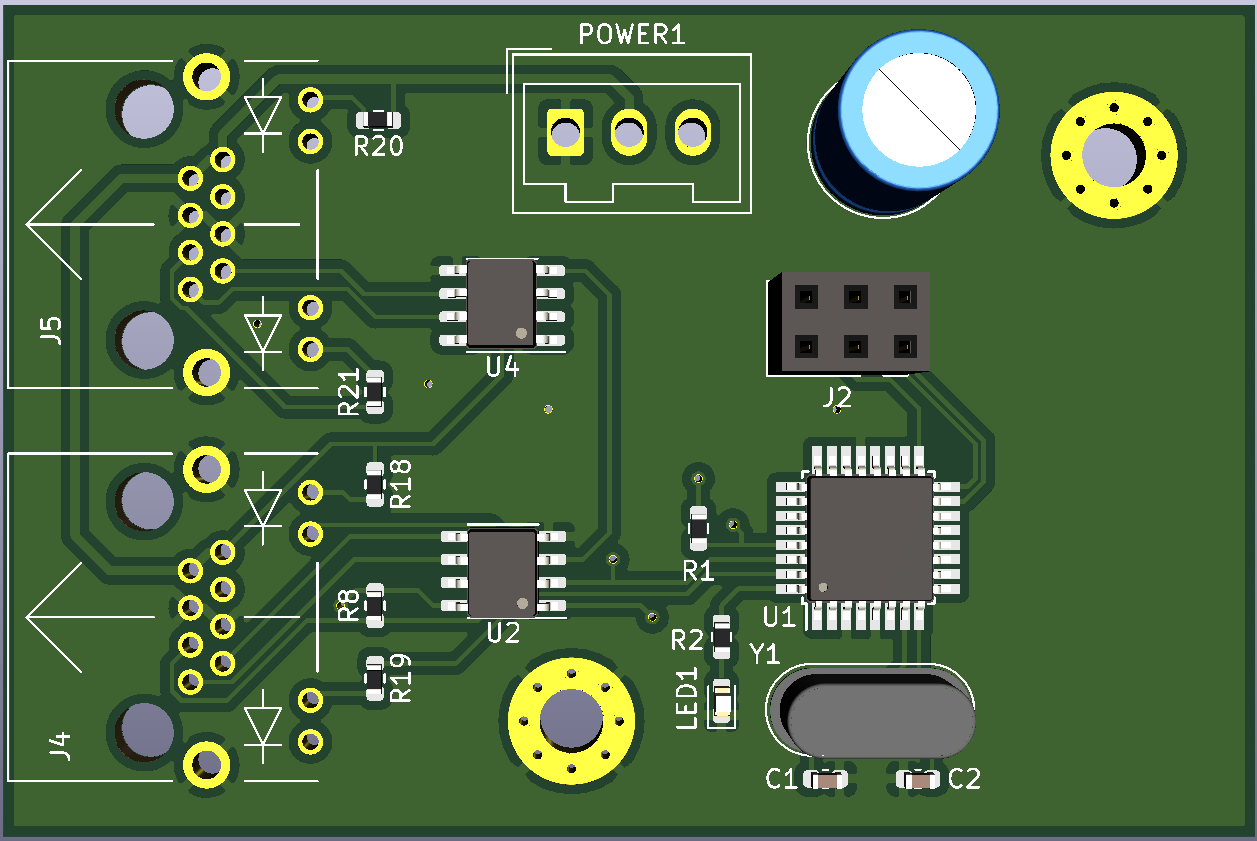
\includegraphics[width=0.6\textwidth]{controller}
    \caption{controller board (CTRB)}
    \label{fig:ctrb}
\end{figure}

The \emph{controller board} (CTRB) is the simplest of the PCB designs currently in use.
It only contains a power connector (\texttt{POWER1}), a microcontroller with the associated circuitry and 2 RJ45 connectors with their corresponding transceiver chips.
\texttt{J2} is a mirrored AVR-ICP-6\footnote{in-circuit programming connector used for AVR microprocessors} connector:
The pinout nearly matches a standard AVR-ICP-6 interface, but the top and bottom rows are swapped.

Each RJ45 connector is used for one of the two busses:
\texttt{J4} provides a connection to the \emph{local bus}.
\texttt{J5} is used for the \emph{remote bus}.
It is recommended that this board is always externally powered to provide a power injection point for both busses.

\section{I/O Interface Board}
\begin{figure}[h!]
    \centering
    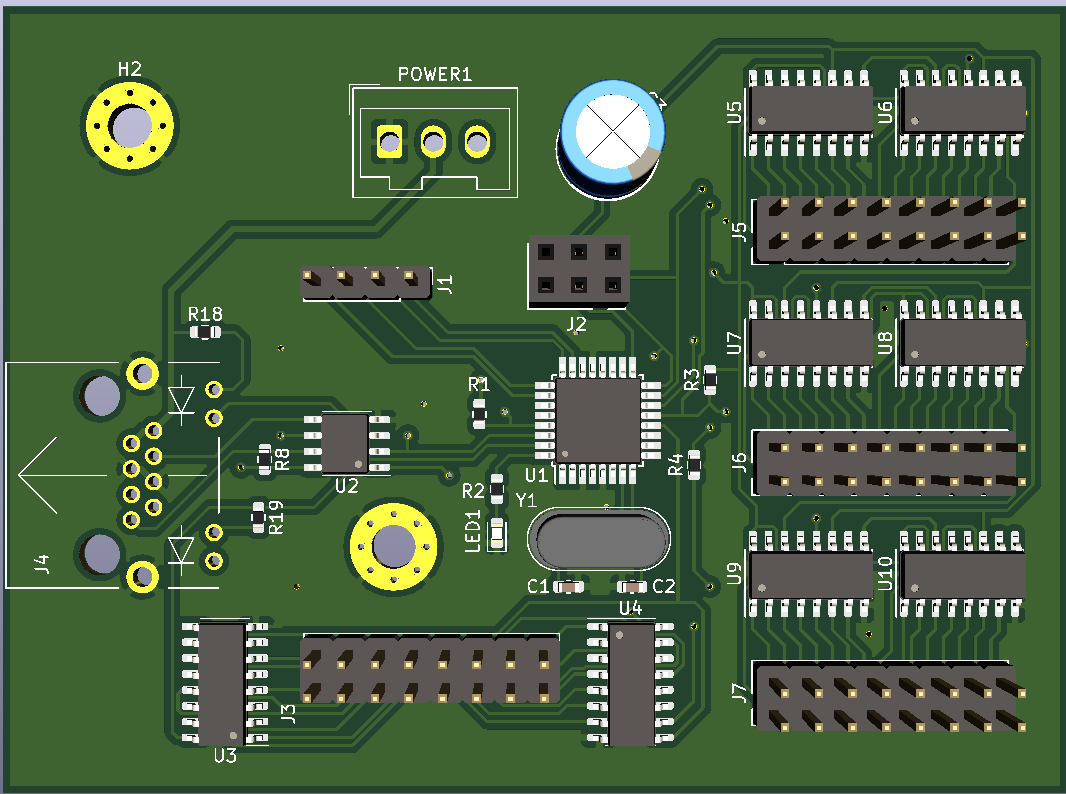
\includegraphics[width=0.8\textwidth]{interface}
    \caption{I/O interface board (IOIB)}
\end{figure}

The \emph{I/O interface board} (IOIB) monitors the push-buttons and drives the LEDs of the control panel.

The \texttt{POWER1} and \texttt{J2} connector are identical to those on the CTRB.
The singular RJ45 connector \texttt{J4} connects to the \emph{local bus}.
The remaining connectors handle \emph{input} and \emph{output}.

\subsection{Input Connectors}
The control panel buttons are divided into 4 sectors of up to 16 buttons each.
The IOIB regularly scans all 4 sectors individually.

The buttons need to be wired in a very specific way:
Each sector has a common \emph{feed pin}.
One terminal of all buttons in one sector needs to be tied to this \emph{feed pin}.
The second terminal is connected to one of the 16 \emph{sense pins} through a series diode.
This diode needs to be oriented with the anode connected to the button and the cathode to the sense pin.
This arrangement leads to a button matrix where for every combination of feed pin sense pin there is exactly one button between these two.
That way when powering the feed pin of one sector the sense pins of all currently pressed buttons of that sector are powered.

The 4-pin connector \texttt{J1} exposes the 4 feed pins for the 4 sectors.
The 16-pin connector \texttt{J3} exposes the 16 sense pins.
All pins of \texttt{J3} require an external pull-down resistor:
The sense pins do posses some stray capacitance.
Due to the diode arrangement residual charges may not dissipate sufficiently quickly through leakage currents alone.
A relatively high resistance\footnote{about $10k\Omega$ should work fine} should be used to not overload the button diodes.

\subsubsection{Button Addressing}
The following simple formula provides a simple way to calculate the button address from a combination of a feed pin and a sense pin:
\[addr = 16 * (feed - 1) + sense - 1\]

Example:
Button 4 of sector 2 would have the button id $0x13$.\footnote{pin numbers are 1-indexed}

\subsection{Output Connectors}
The remaining connectors (\texttt{J5}, \texttt{J6} and \texttt{J7}) handle \emph{output} - \emph{i.e.} the control panel LEDs.
Each connector provides signals for 16 LEDs.
These pins are directly connected to the 74HC595 shift registers.
While low-power devices could be directly connected to these digital pins it is recommended to use these pins only to drive the gates on external NMOS transistors.
In that configuration the NMOS does not require a pull-down resistor on the gate pin as the IOIB pins are always actively driven.

The 3 connectors are arranged in software as 6 bytes of data.
\texttt{J5} exposes the 2 least significant bytes while \texttt{J7} exposes the 2 most significant bytes.
On each connector pin 1 is the least significant bit of the less significant byte.
\begin{table}[h!]
\centering
\begin{tabular}{ |c|c|c|c|c|c| } \hline
\multicolumn{2}{ |c| }{\texttt{J5}} & \multicolumn{2}{ |c| }{\texttt{J6}} & \multicolumn{2}{ |c| }{\texttt{J7}} \\\hline
pins 1-8 & pins 9-16 & pins 1-8 & pins 9-16 & pins 1-8 & pins 9-16  \\\hline\hline
$data_0$ & $data_1$  & $data_2$  & $data_3$  & $data_4$  & $data_5$ \\\hline
\end{tabular}
\caption{output pin assignments}
\end{table}

\pagebreak
\section{Decoder Boards}
The decoder boards share much of the basic hardware.
Specifically the power connector, the programming header and the 2 RJ45 connectors are all arranged identically on all decoders.
Also the microprocessor and all basic support components share common placement and trace routing.

\begin{figure}[h!]
    \centering
    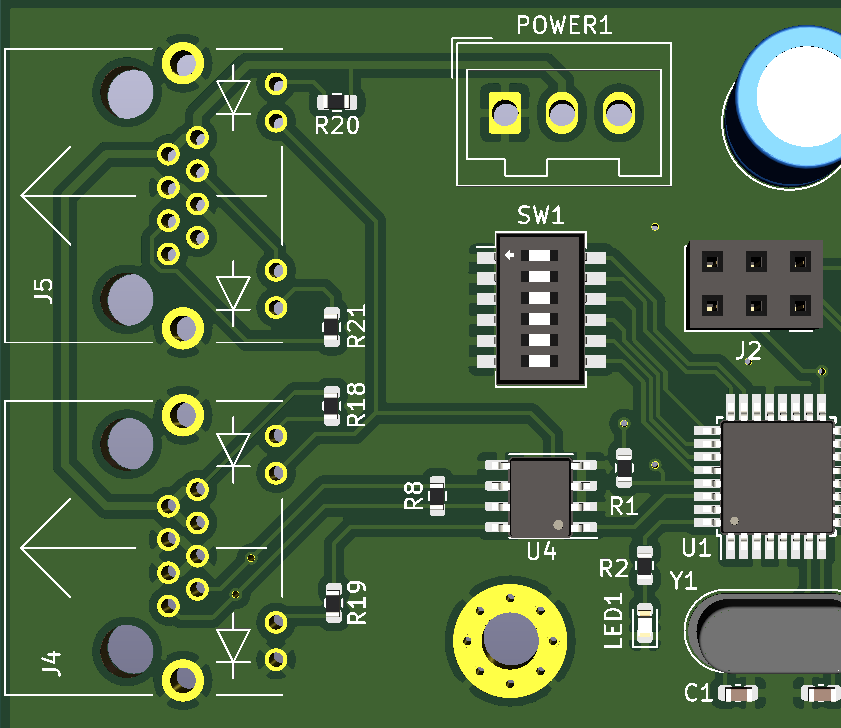
\includegraphics[width=0.4\textwidth]{decoder_general}
    \caption{common area of decoder PCBs}
\end{figure}

On the decoder boards the 2 RJ45 connectors are used for daisy chaining the \emph{remote} bus.
The connector \texttt{J4} is used as the \emph{input} -- \emph{i.e.} the connection to the CTRB or a \emph{previous} board.
The second connector -- \texttt{J5} -- is the \emph{output}.
This connector is used to connect to the \emph{next} board in the chain.
At the last board in the chain this connector can simply be left disconnected and no bus termination is required.

The power connector (\texttt{POWER1}) can be used to externally power the decoder and to provide power to the bus.
On low-power boards it can be left unpopulated or disconnected.

The 6-channel DIP-switch \texttt{SW1} can be used to provide configuration data to the microprocessor.
This could -- for example -- be used to configure the decoder type and address.
The header is provided on all decoders but is not required to be populated if not needed by a decoder.

Please note that the mounting holes are plated and the plating is connected to the ground plane of the board.
To ensure balanced currents on the bus power wires it is recommended to ensure that the mounting screws -- and thereby the mounting holes -- remain electrically isolated from any external ground connection on boards that are bus powered.
On externally powered boards this isolation is not required.

\pagebreak
\subsection{General Purpose Decoder}
\begin{figure}[h!]
    \centering
    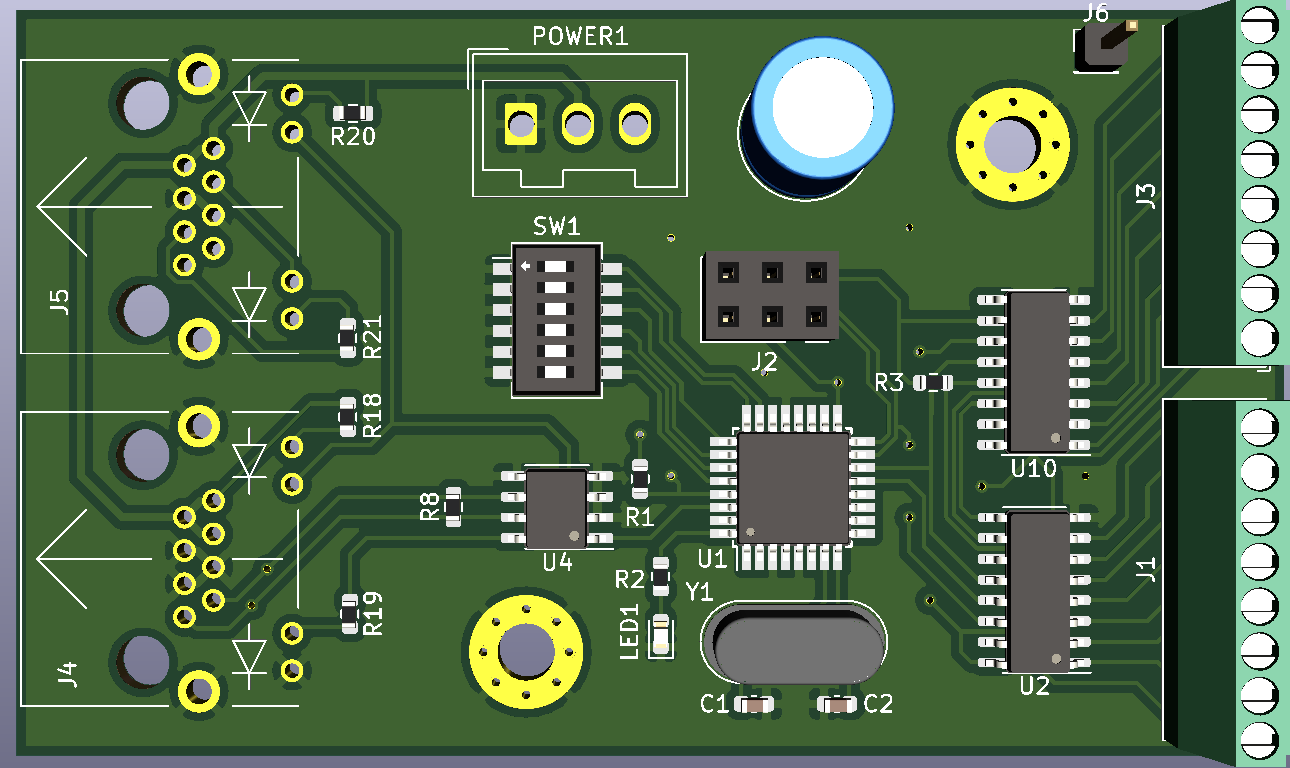
\includegraphics[width=0.6\textwidth]{common_decoder}
    \caption{general purpose decoder board}
\end{figure}

Many functions of the control system require simple digital -- or low-power -- pins.
The \emph{general purpose decoder} provides a generic hardware platform for all these uses.
It is the simplest of the decoder boards and is used for all signal decoders and for lighting.
This board exposes up to 16 pins that are directly wired to the parallel output of two 74HC595 shift registers.
The pins do have tri-state support.
This feature can of course be controlled by the individual decoder software.

The connectors \texttt{J1} and \texttt{J3} expose the 16 output pins.
\texttt{J1} holds the first 8 pins, \texttt{J3} the rest.
In a situation where less than 9 pins are used the header \texttt{J3} and 
the shift register \texttt{U10} can remain unpopulated.
When using the output pins to directly power external components it must be ensured that each pin does not exceed the maximum pin current and each connector does not exceed the maximum port current for the specific shift register used.
Power usage should probably be kept below $10mA$ per pin.

In some situation the output pins may be used as open collectors to power low power devices (\emph{e.g.} LEDs).
These do require a power supply.
If the board is bus-powered the power supply to the external devices should also be taken from the board to keep the currents through the power cables on the bus balanced.
The power may either be taken from the \texttt{POWER1} connector or from the auxiliary pin \texttt{J6} which is also connected to the 5V rail of the board.

\pagebreak
\subsection{Switch Decoder}
\begin{figure}[h!]
    \centering
    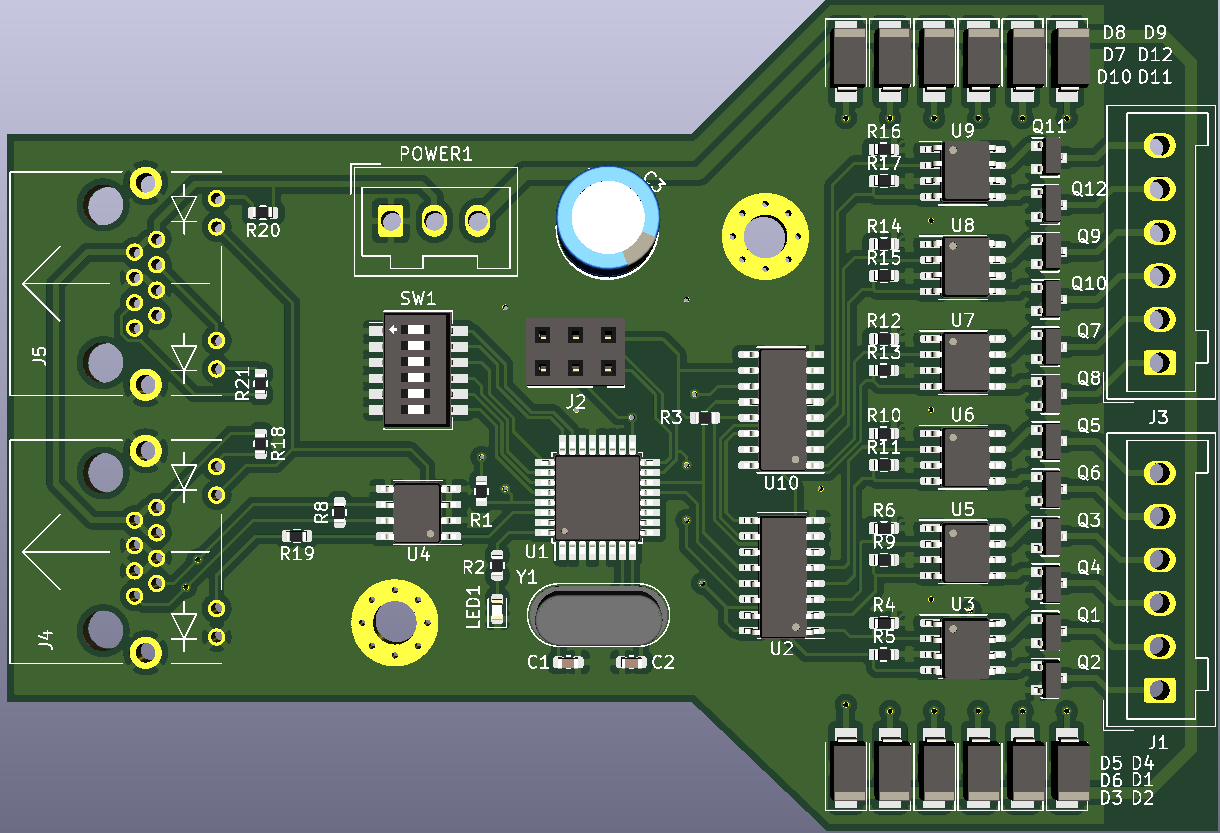
\includegraphics[width=0.7\textwidth]{switch_decoder}
    \caption{switch decoder board}
\end{figure}

Currently the only decoder type with bespoke hardware is the switch decoder.
Each switch decoder allows control of up to 6 switches.

\texttt{J1} and \texttt{J3} provide open collector connections for 3 switches each.
The first pin of each switch should always be connected to the motor pole that pulls the switch into the \emph{straight-through} position.

Each pin is switched to ground through an NMOS transistor with a MOSFET driver IC to minimise switching times.
In addition each pin is also connected to a flyback diode.
Switch motors are usually inductive loads and when switching of a motor pole a voltage spike may occur that could be destructive to the switching transistor.
The on-board high-current schottky diodes protect the transistors from any such voltage spikes.

A connection to the power supply voltage of the switches is required for the flyback diodes to work properly.
The generally unused third pin of the power connector (\texttt{POWER1}) is connected to the cathode of all flyback diodes.
It should be connected to the 24V power rail powering the switches.
Failure to connect the 24V rail could lead to destructive failure of the NMOS transistors due to the drain-source voltage exceeding its limit.
For this reason it is recommended to verify a stable connection upon installation.
A voltage measurement between the cathode of any flyback diode and an exposed mounting hole plating can be used for this purpose.

If a decoder does not control 6 switches, the components for any unused connections can remain unpopulated.
A single switch is driven by one dual-channel MOSFET driver with one pull-down resistor per channel and two NMOS transistors with a flyback diode each.

\chapter{Decoder Command Specification}
Each decoder type has its own command structure.
These decoder command structures in essence define an \emph{instruction set} of instructions sent from the CTRB to the decoders to control the model railway.
The following sections provide detailed specifications for all currently supported commands.

\section{Switch Commands}

\section{Exit Signal Commands}

\section{Entry Signal Commands}

\section{Lighting Commands}

\end{document}
